\section{Experimental results}
In this section we outline the results obtained by running the simulations in terms of the chosen performance metrics.
\subsection{Algorithm accuracy}
To evaluate the accuracy of the algorithm, we performed five simulations for each of the five fitness functions while maintaining a fixed number of iterations and population size. For the Sphere, McCormick, Matyas, and Michalewicz functions, we used the default optimization parameters \cite{pepo}. In all simulations, the algorithm successfully converged and found the actual optimal value.  
\newline
However, for the Bukin function, due to its complexity and the presence of numerous local minima, we increased the population size to 400 and set the exploration parameter to 3. Despite these adjustments, the algorithm was still unable to consistently converge in all simulations, as it frequently became trapped in one of the many local minima.  
\newline
For consistency, we reported the deviation from the actual optimal value obtained in the different simulations, as shown in Figure~\ref{fig:bukin_deviation}.
\newline
\begin{figure}[h]
    \centering
    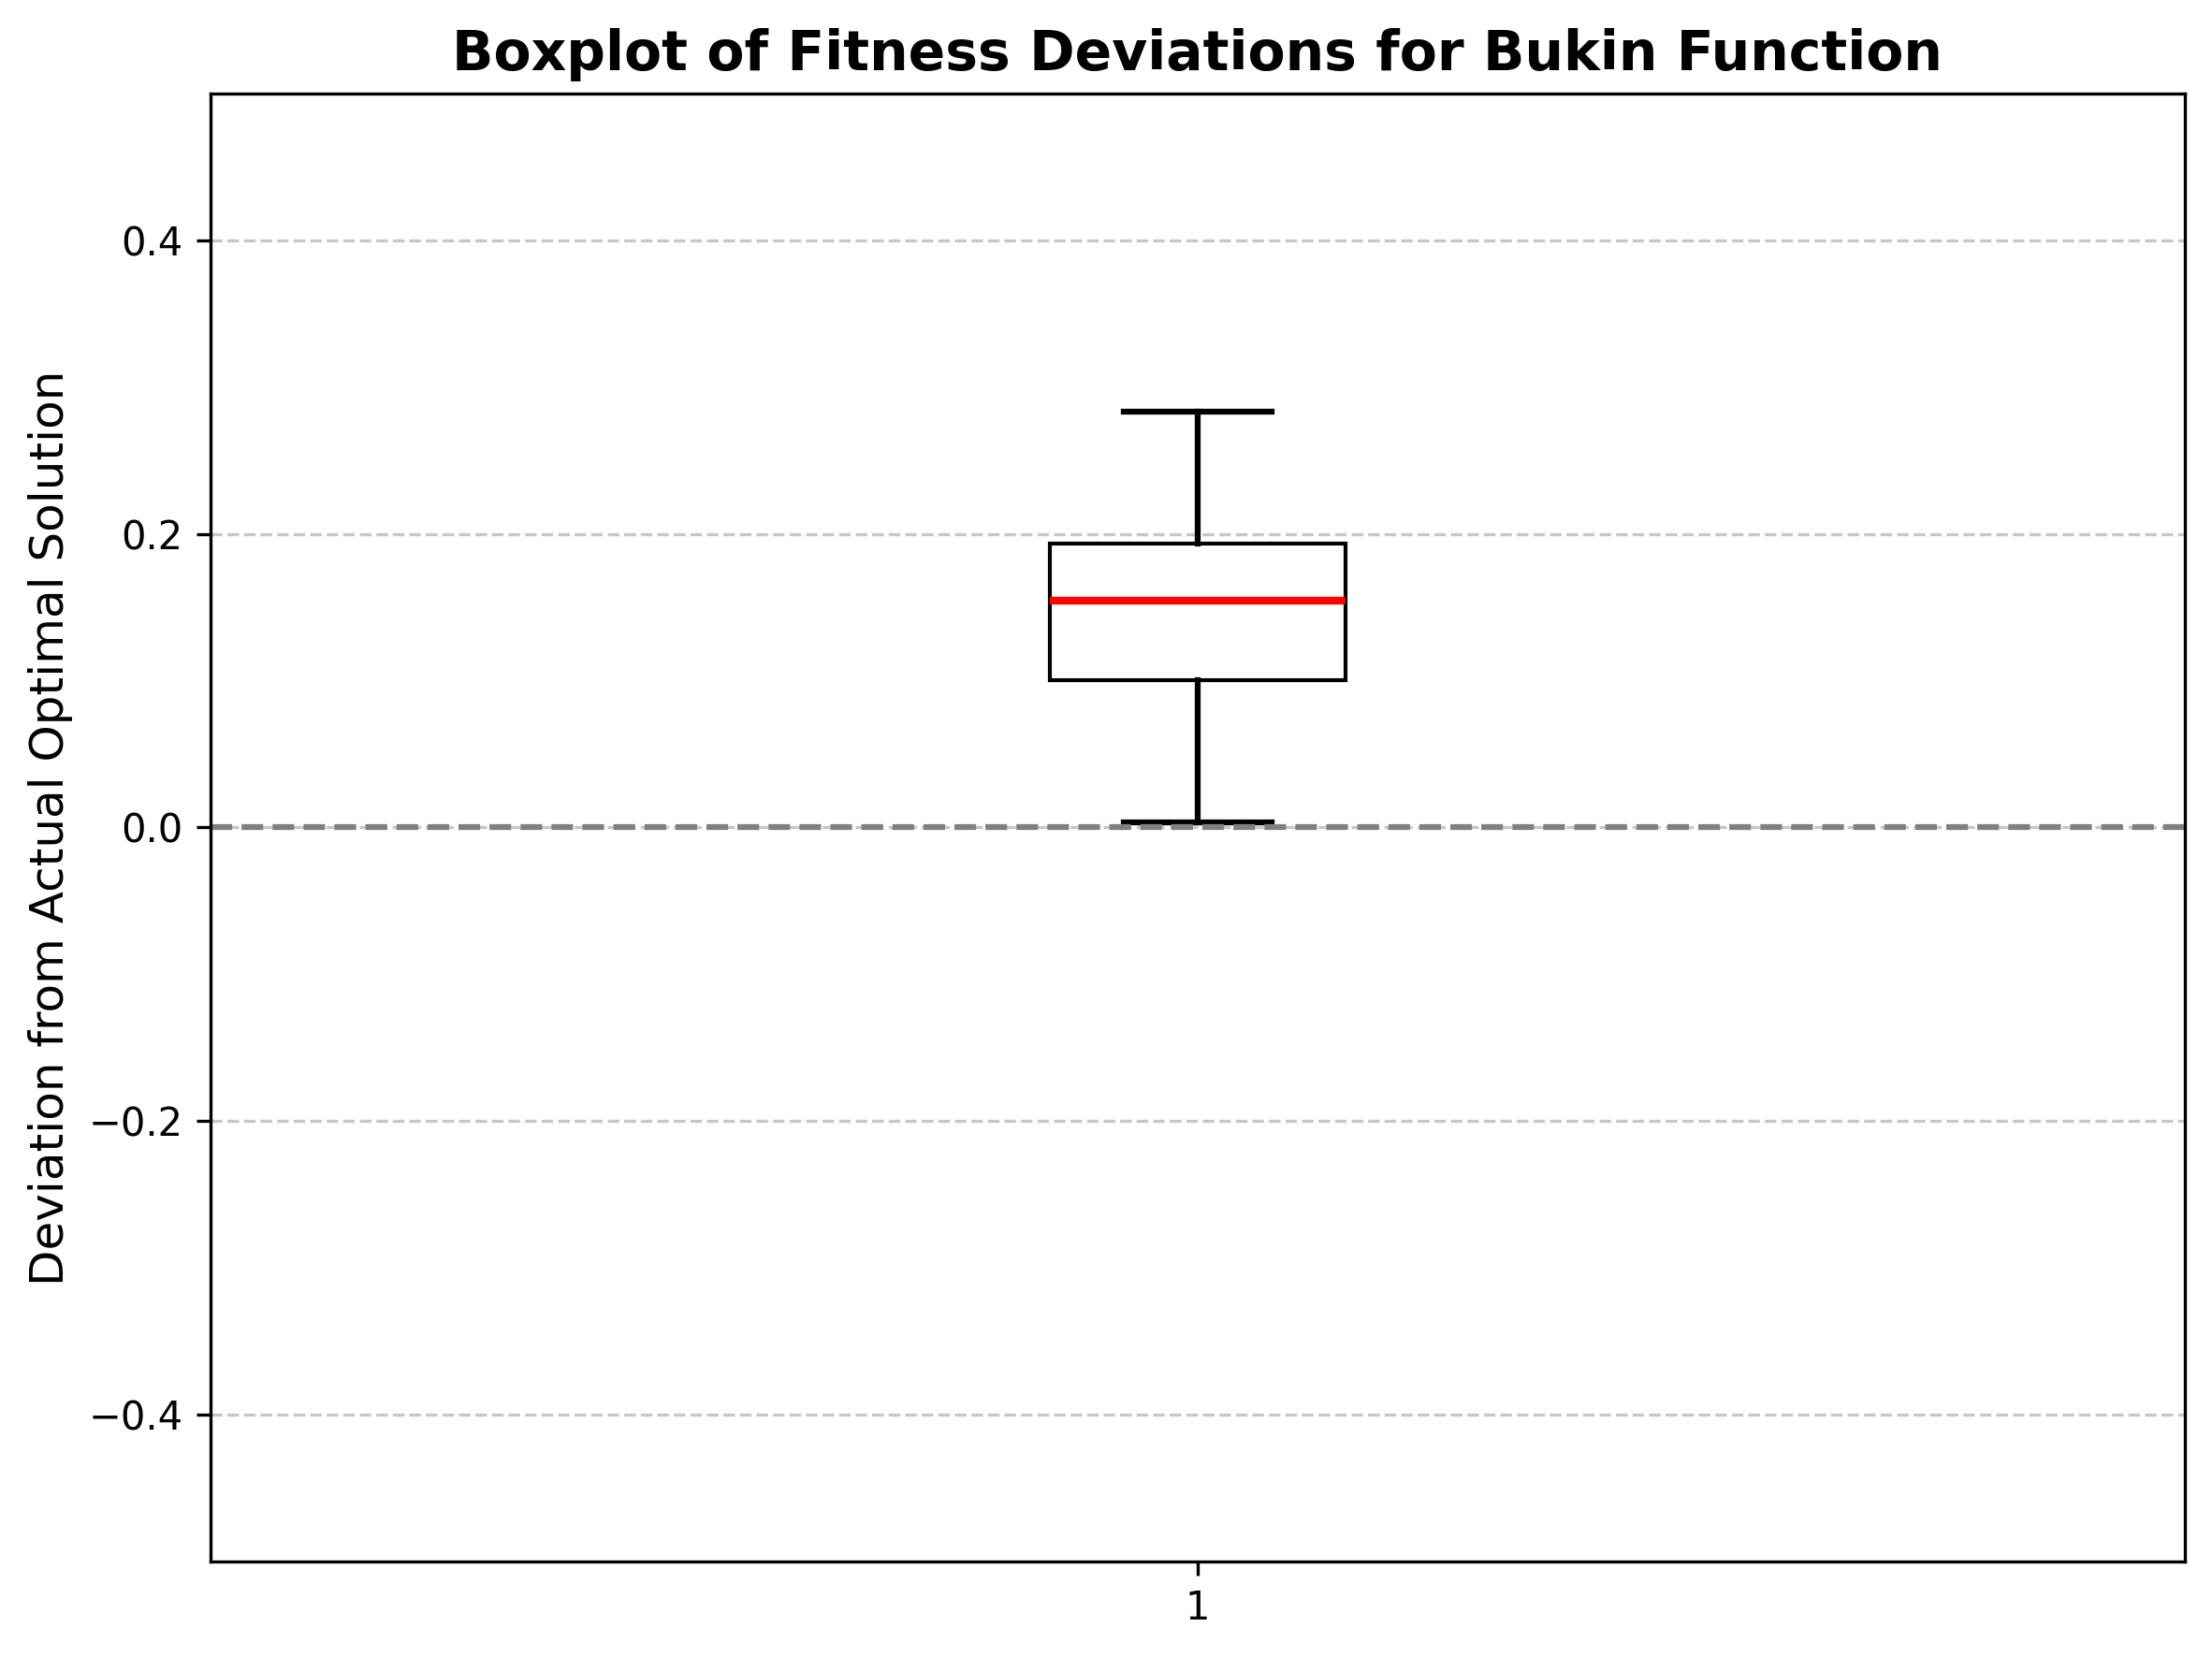
\includegraphics[width=0.5\textwidth]{figures/bukin_fitness_boxplot.png} % Adjust file name if necessary
    \caption{Deviation from the optimal value for the Bukin function.}
    \label{fig:bukin_deviation}
\end{figure}
\newline
\subsection{Parallel performance}
We conducted several simulations of the parallel algorithm, varying the number of nodes and threads from 1 to 50 and the population size. Since our goal was to analyze parallelization performance, we considered the optimization parameters to be irrelevant in this context.  
\newline
For consistency, we kept the number of variables fixed at 100, used the Sphere function, and set a constant number of iterations at 500. We will first outline the results obtained with a varying number of nodes, without considering threads.
\subsubsection{Speedup}
Figure ~\ref{fig:nodes_speedup} illustrates the speedup with different problem sizes while increasing the number of nodes.
\newline
\begin{figure}[h]
    \centering
    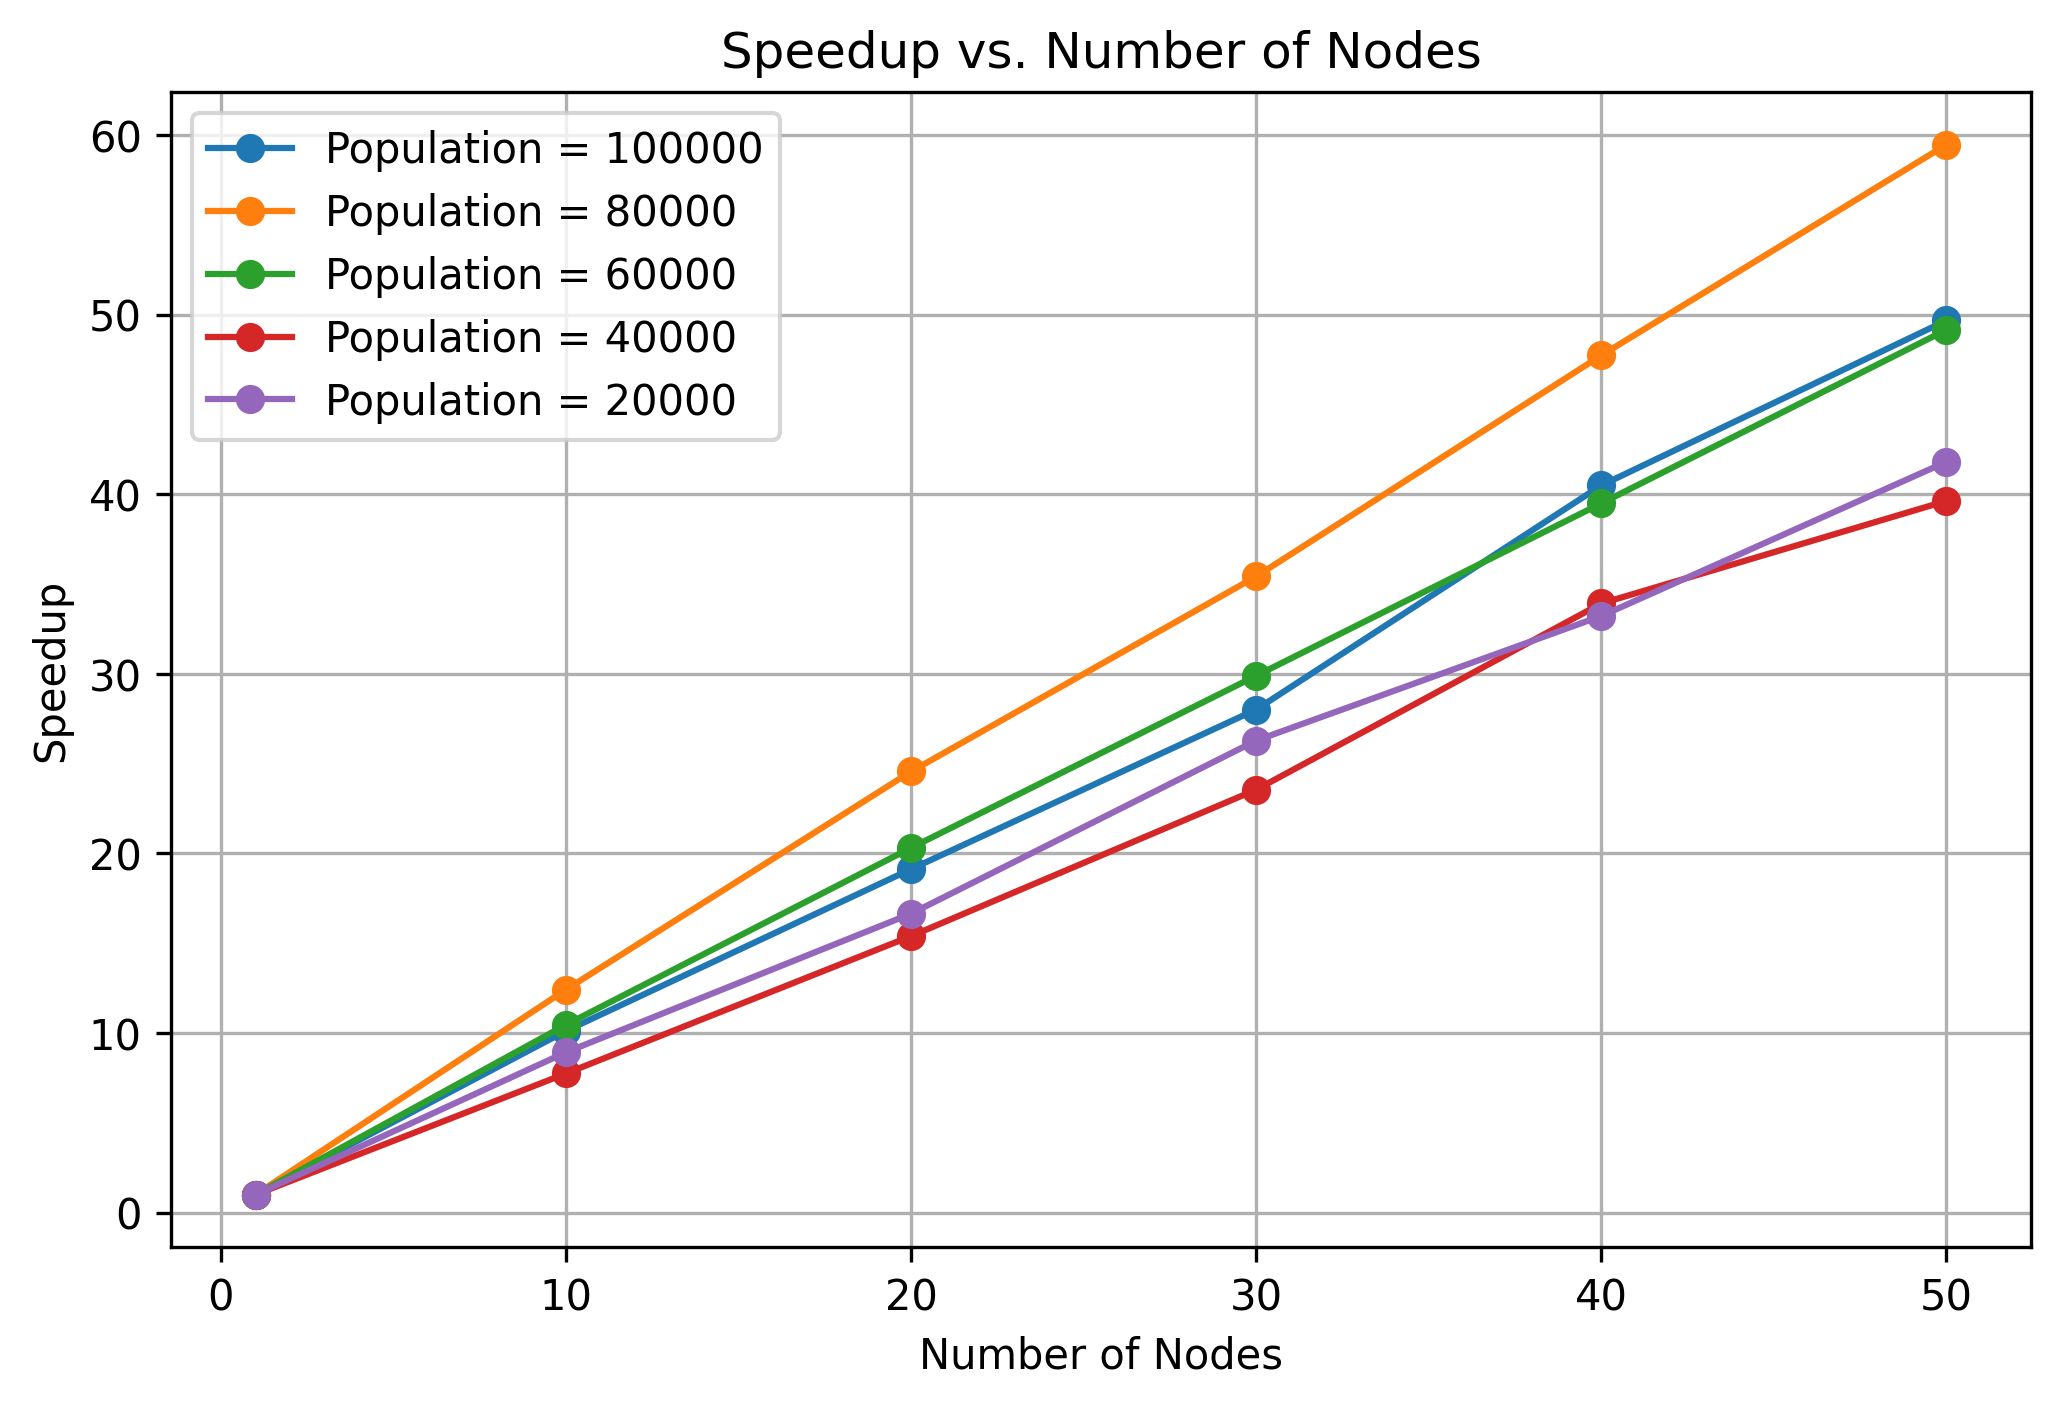
\includegraphics[width=0.5\textwidth]{figures/speedup_vs_nodes.png} % Adjust file name if necessary
    \caption{Speedup graph for different population sizes.}
    \label{fig:nodes_speedup}
\end{figure}
The observed speedup confirms that parallelization effectively reduces the execution time, especially when larger population sizes are used. The speedup increases almost linearly with the number of nodes, which is a strong indicator of good parallel performance.
The different population sizes generally follow a similar trend, though the population of 80,000 shows the highest speedup. This suggests that some problem sizes benefit more from parallelization, potentially due to better workload distribution.
A slight deviation from perfect linear scaling at higher node counts suggests that communication overhead or other bottlenecks might start playing a role.

\subsubsection{Efficiency}
Figure ~\ref{fig:nodes_efficiency} illustrates the efficiency with different problem sizes while increasing the number of nodes.
\newline
\begin{figure}[h]
    \centering
    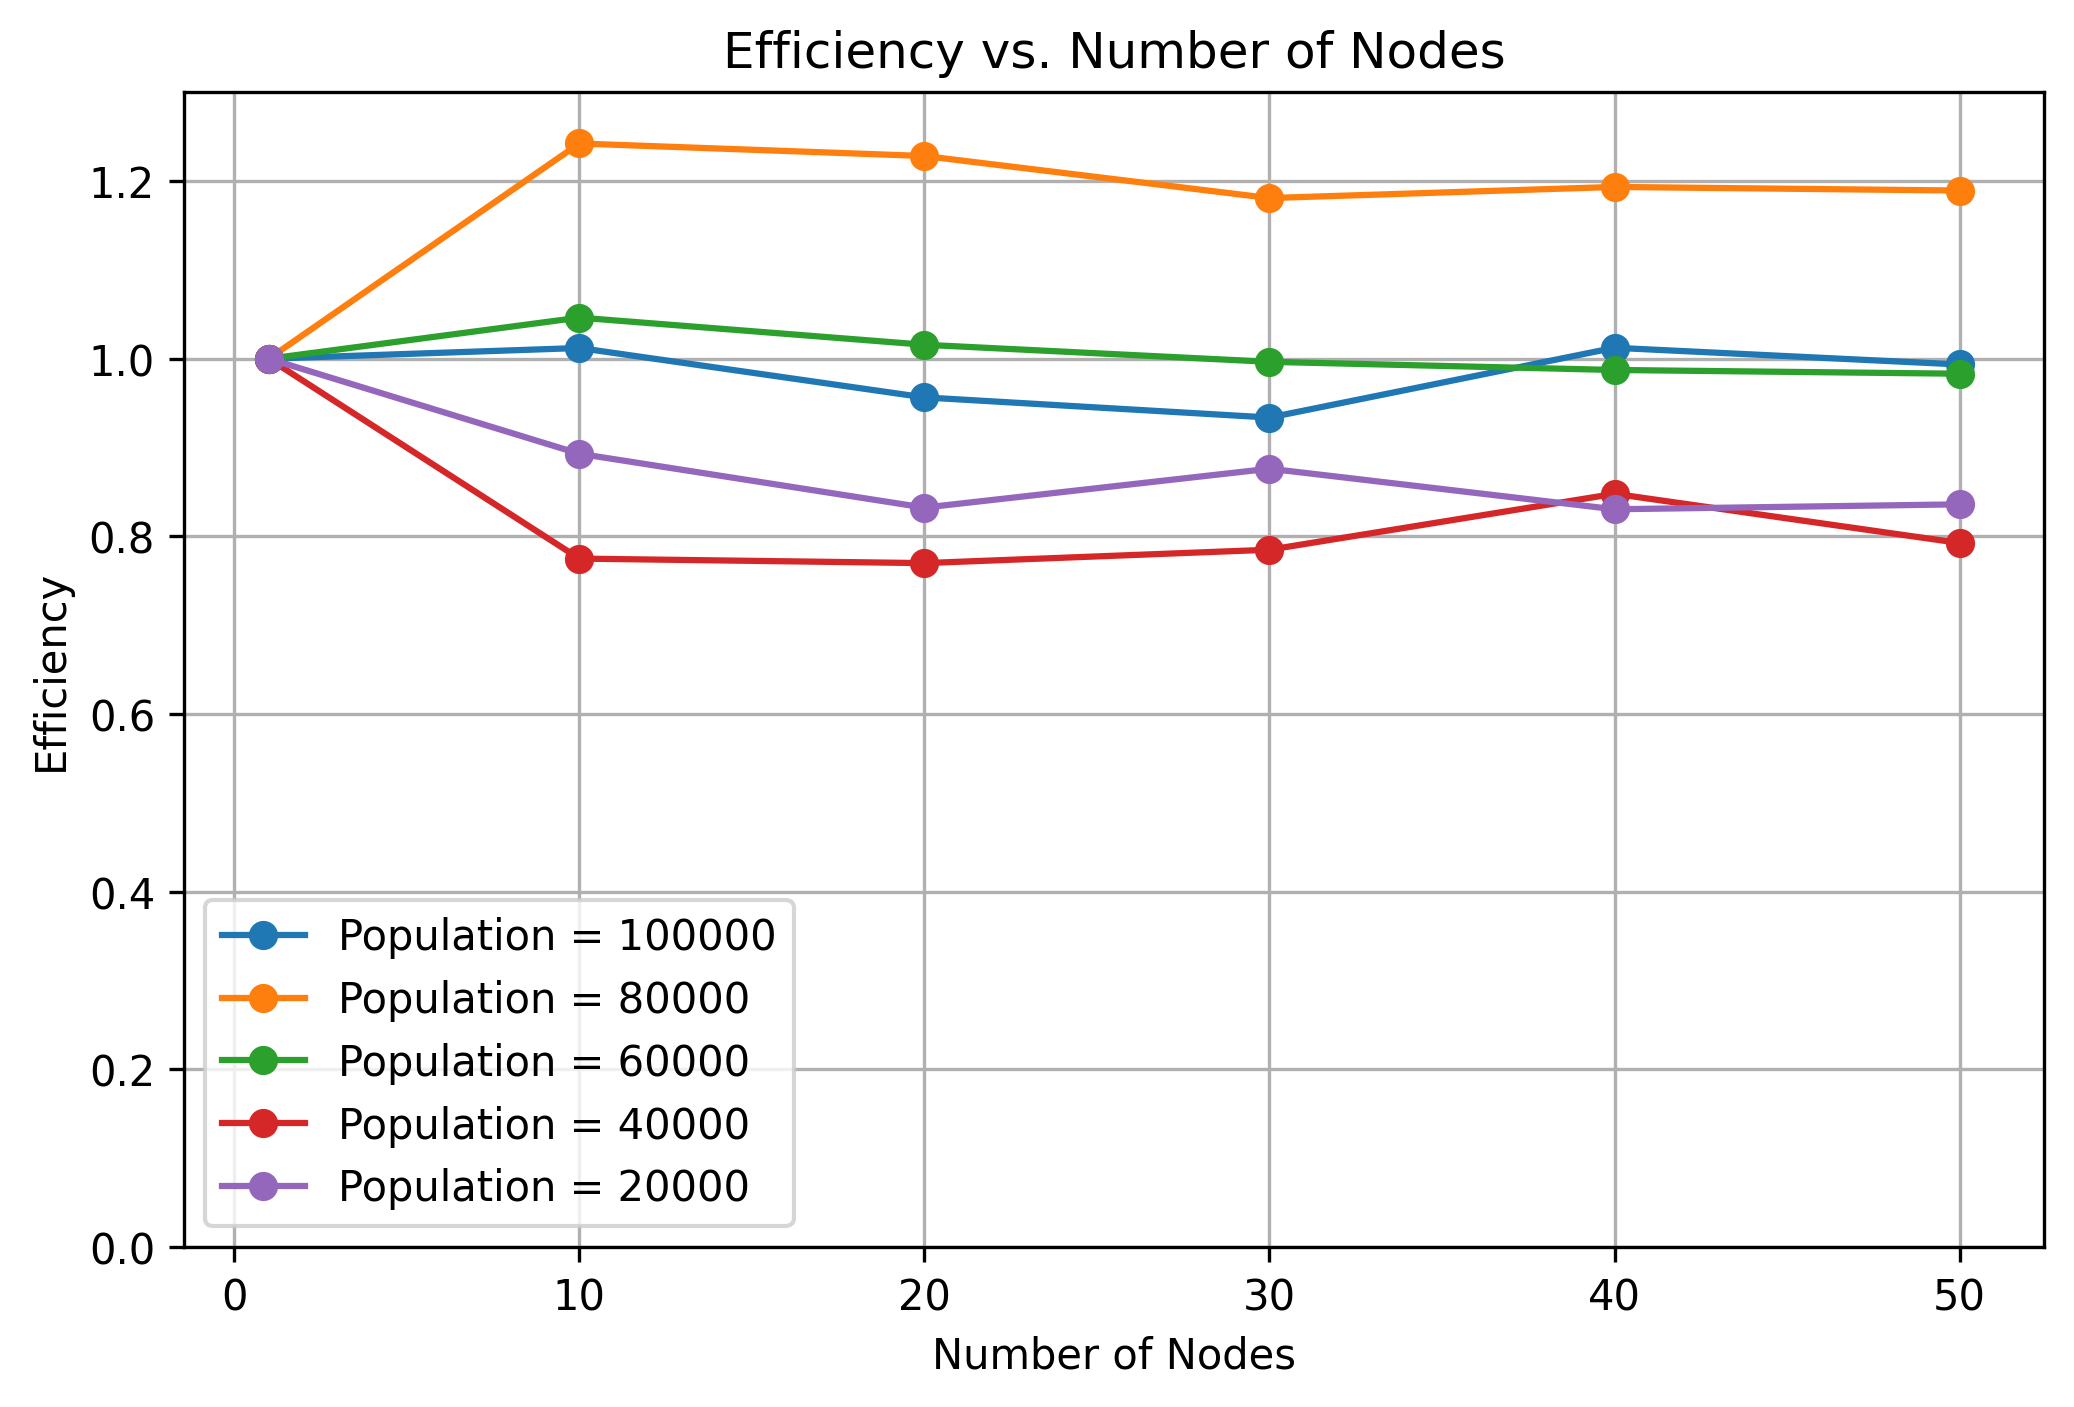
\includegraphics[width=0.5\textwidth]{figures/efficiency_vs_nodes.png} % Adjust file name if necessary
    \caption{Efficiency graph for different population sizes.}
    \label{fig:nodes_efficiency}
\end{figure}
Efficiency mostly remains above or near 1 for larger problem sizes, which is very promising.
The efficiency for the smallest population sizes (20,000 and 40,000) degrades slightly, indicating that these workloads may be too small to benefit from parallelization at higher node counts.
The fact that the efficiency for a population of 80,000 is above 1 suggests a superlinear speedup. While the specific cause of this behavior is not clear, we hypothesize that the heterogeneity of the cluster and the allocation of resources introduce a certain variability, which in turn can affect performance.
\subsubsection{Scalability}
The algorithm demonstrates good strong scaling, as shown in the speedup graph. Figure ~\ref{fig:nodes_scalability} illustrates the weak scalability while increasing the number of nodes.
\begin{figure}[h]
    \centering
    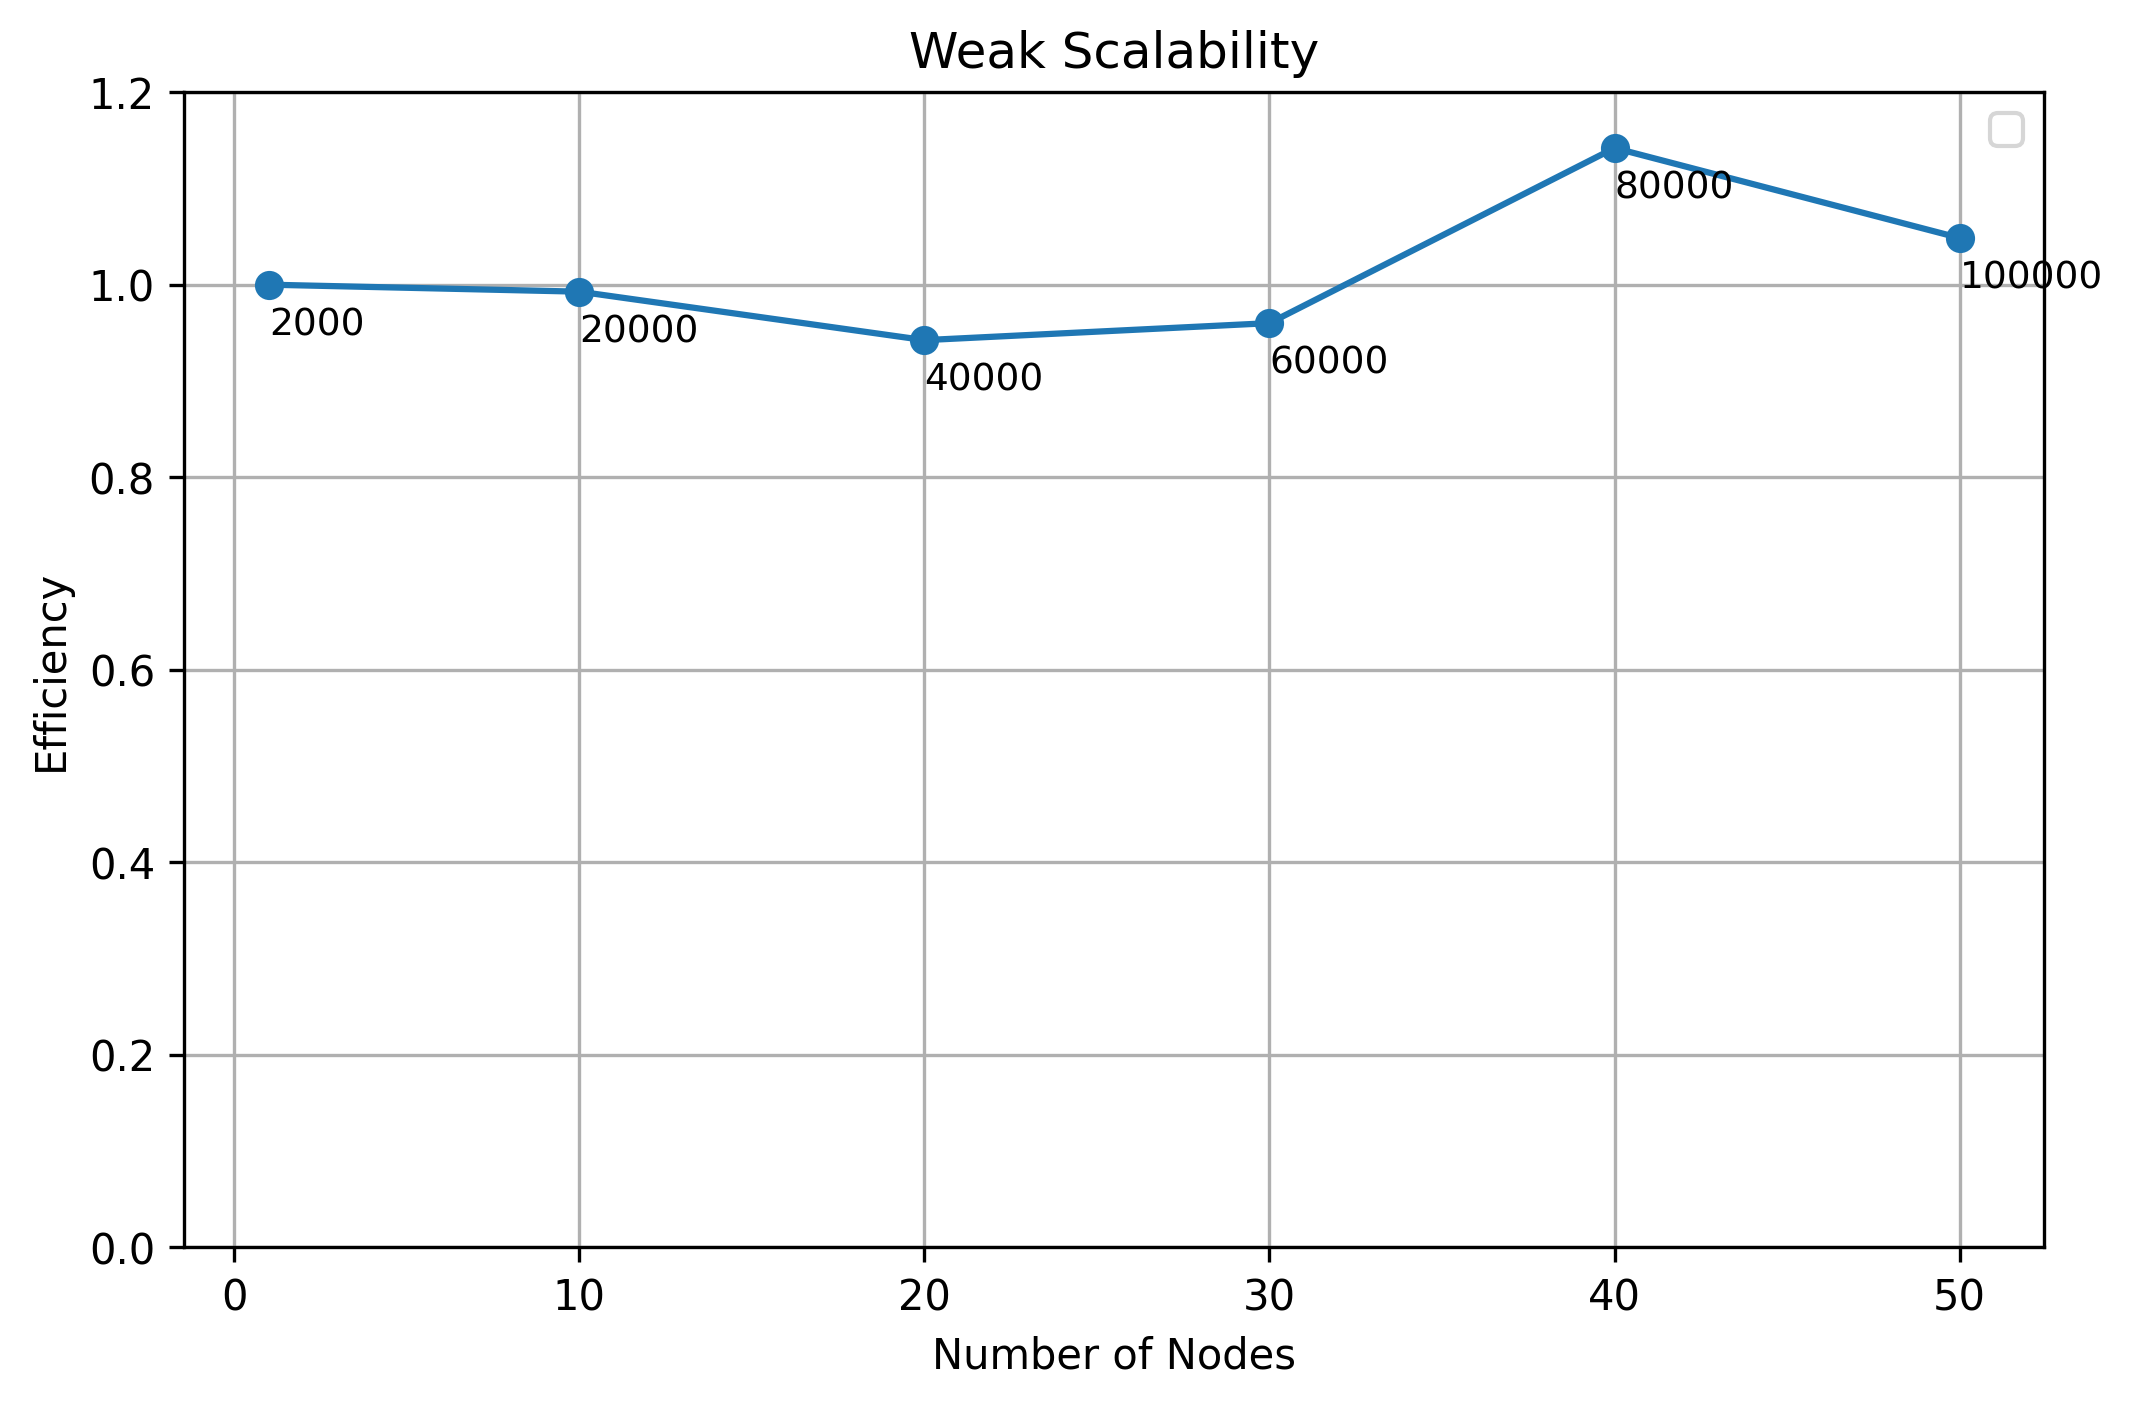
\includegraphics[width=0.5\textwidth]{figures/weak_scalability.png} % Adjust file name if necessary
    \caption{Weak scalability with population size varying from 2000 to 100000}
    \label{fig:nodes_scalability}
\end{figure}
\newline
The efficiency remains around 1 for most cases, which indicates strong weak scaling performance.
A small dip in efficiency around mid-range problem sizes (40,000 and 60,000) suggests potential inefficiencies, but it recovers for the larger problem sizes.
Overall, this result is promising because it indicates that as the problem size grows proportionally with the number of nodes, efficiency remains stable.
\newline
\newline
We conducted the same experiments as with nodes, but using threads to leverage multithreading. However, we observed a degradation in performance. This suggests that our algorithm scales better with distributed computing than with shared-memory parallelism.
\begin{figure}[h]
    \centering
    \begin{subfigure}{0.45\textwidth}
        \centering
        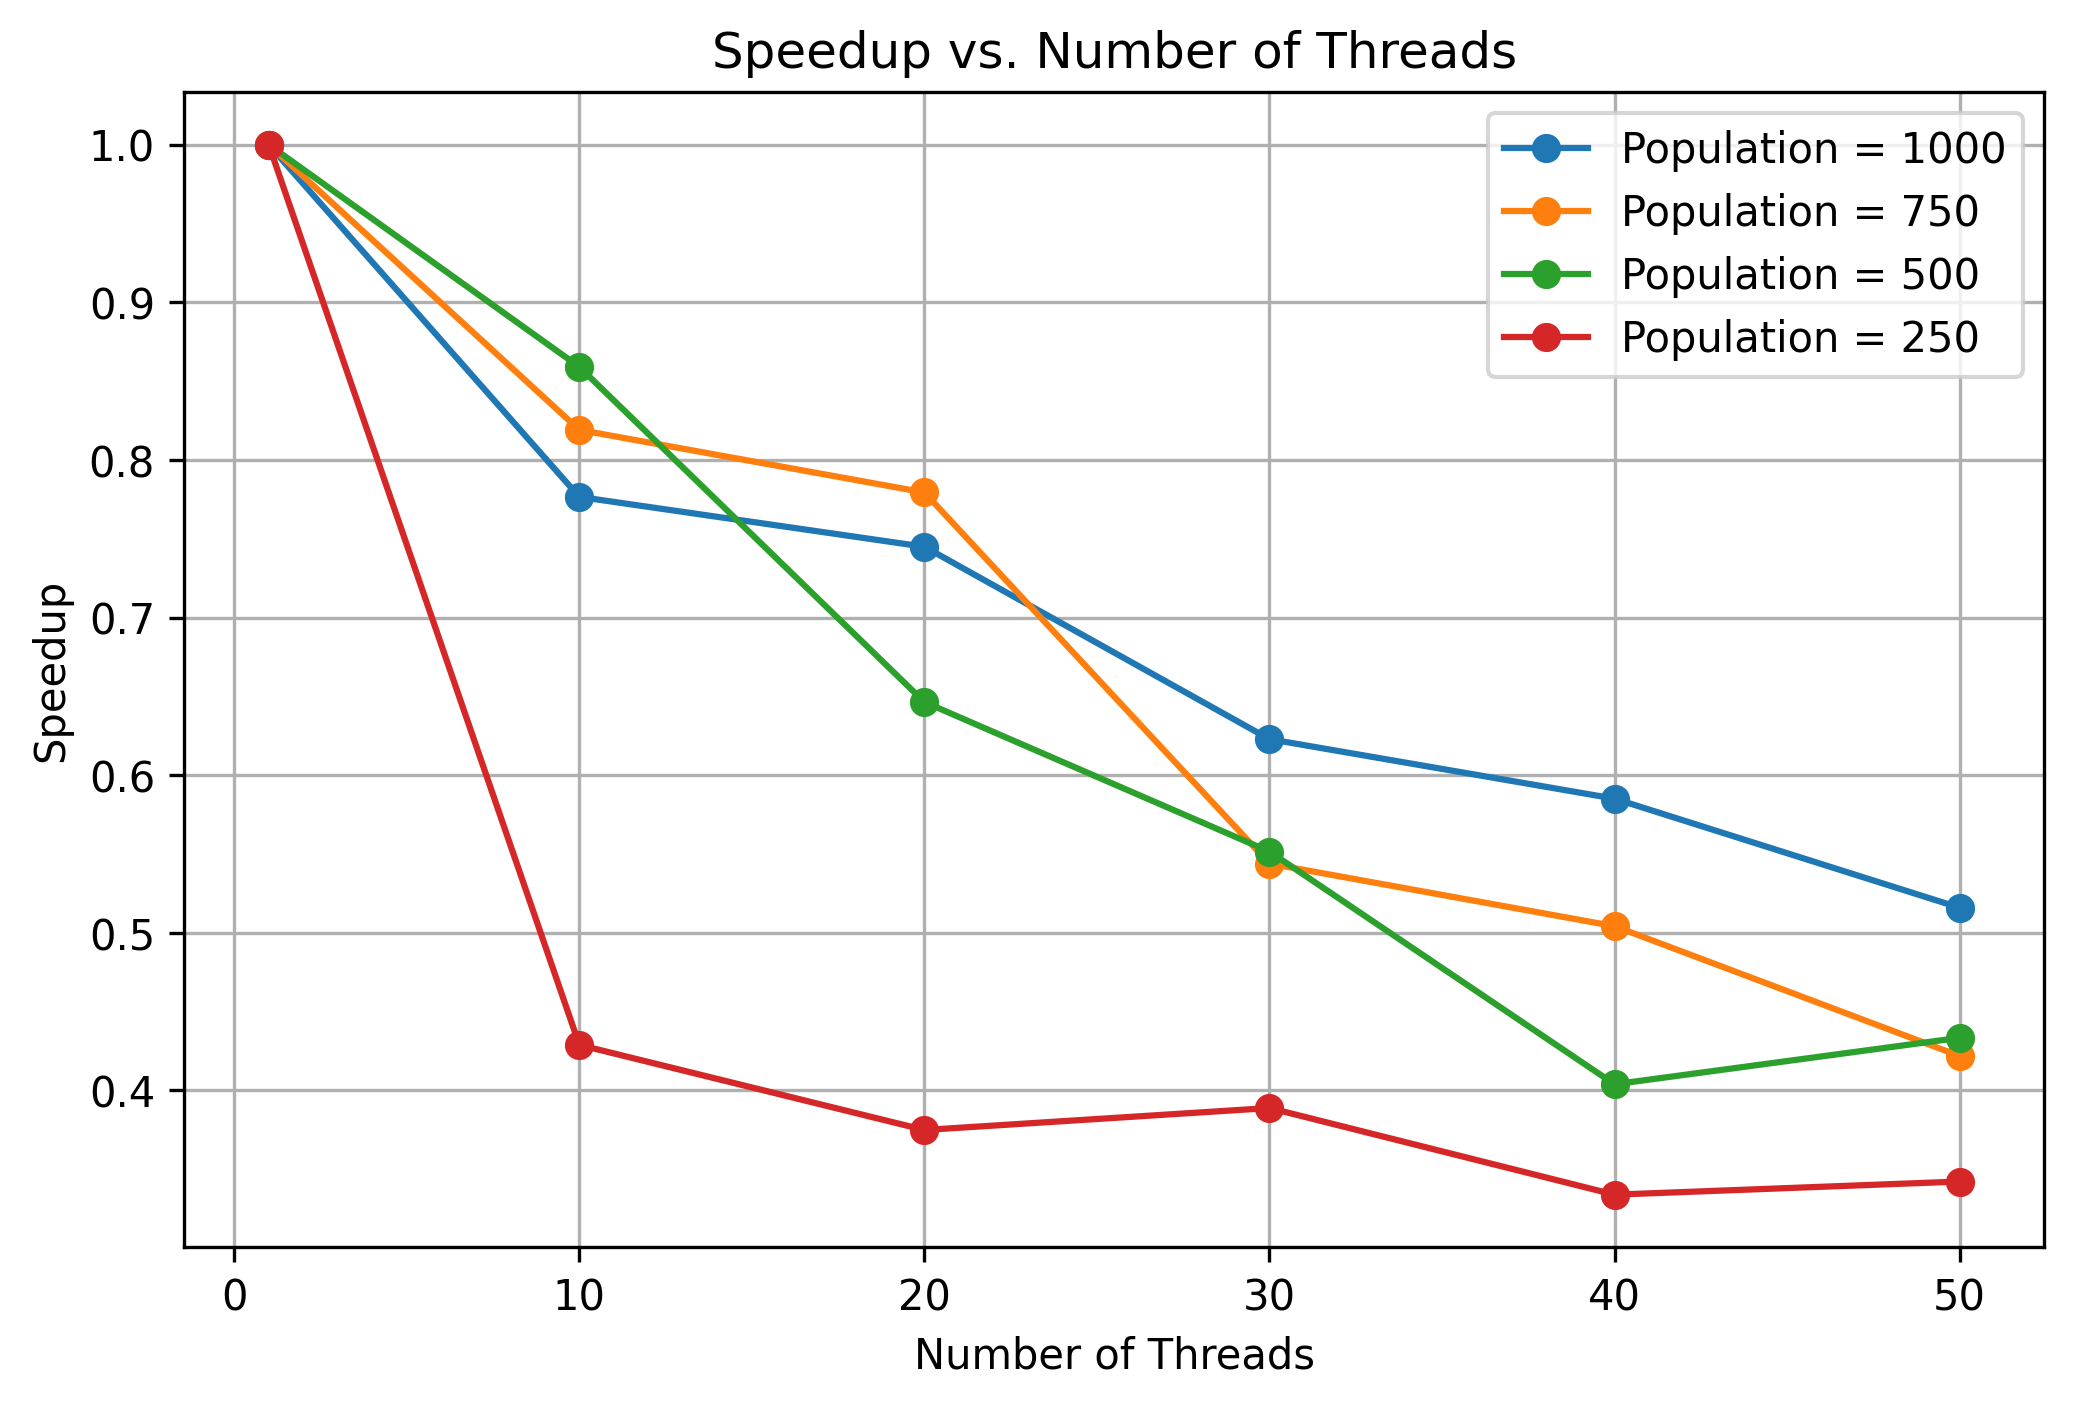
\includegraphics[width=\linewidth]{figures/speedup_vs_threads.png}
        \caption{Speedup vs. Number of Threads}
    \end{subfigure}
    \hfill
    \begin{subfigure}{0.45\textwidth}
        \centering
        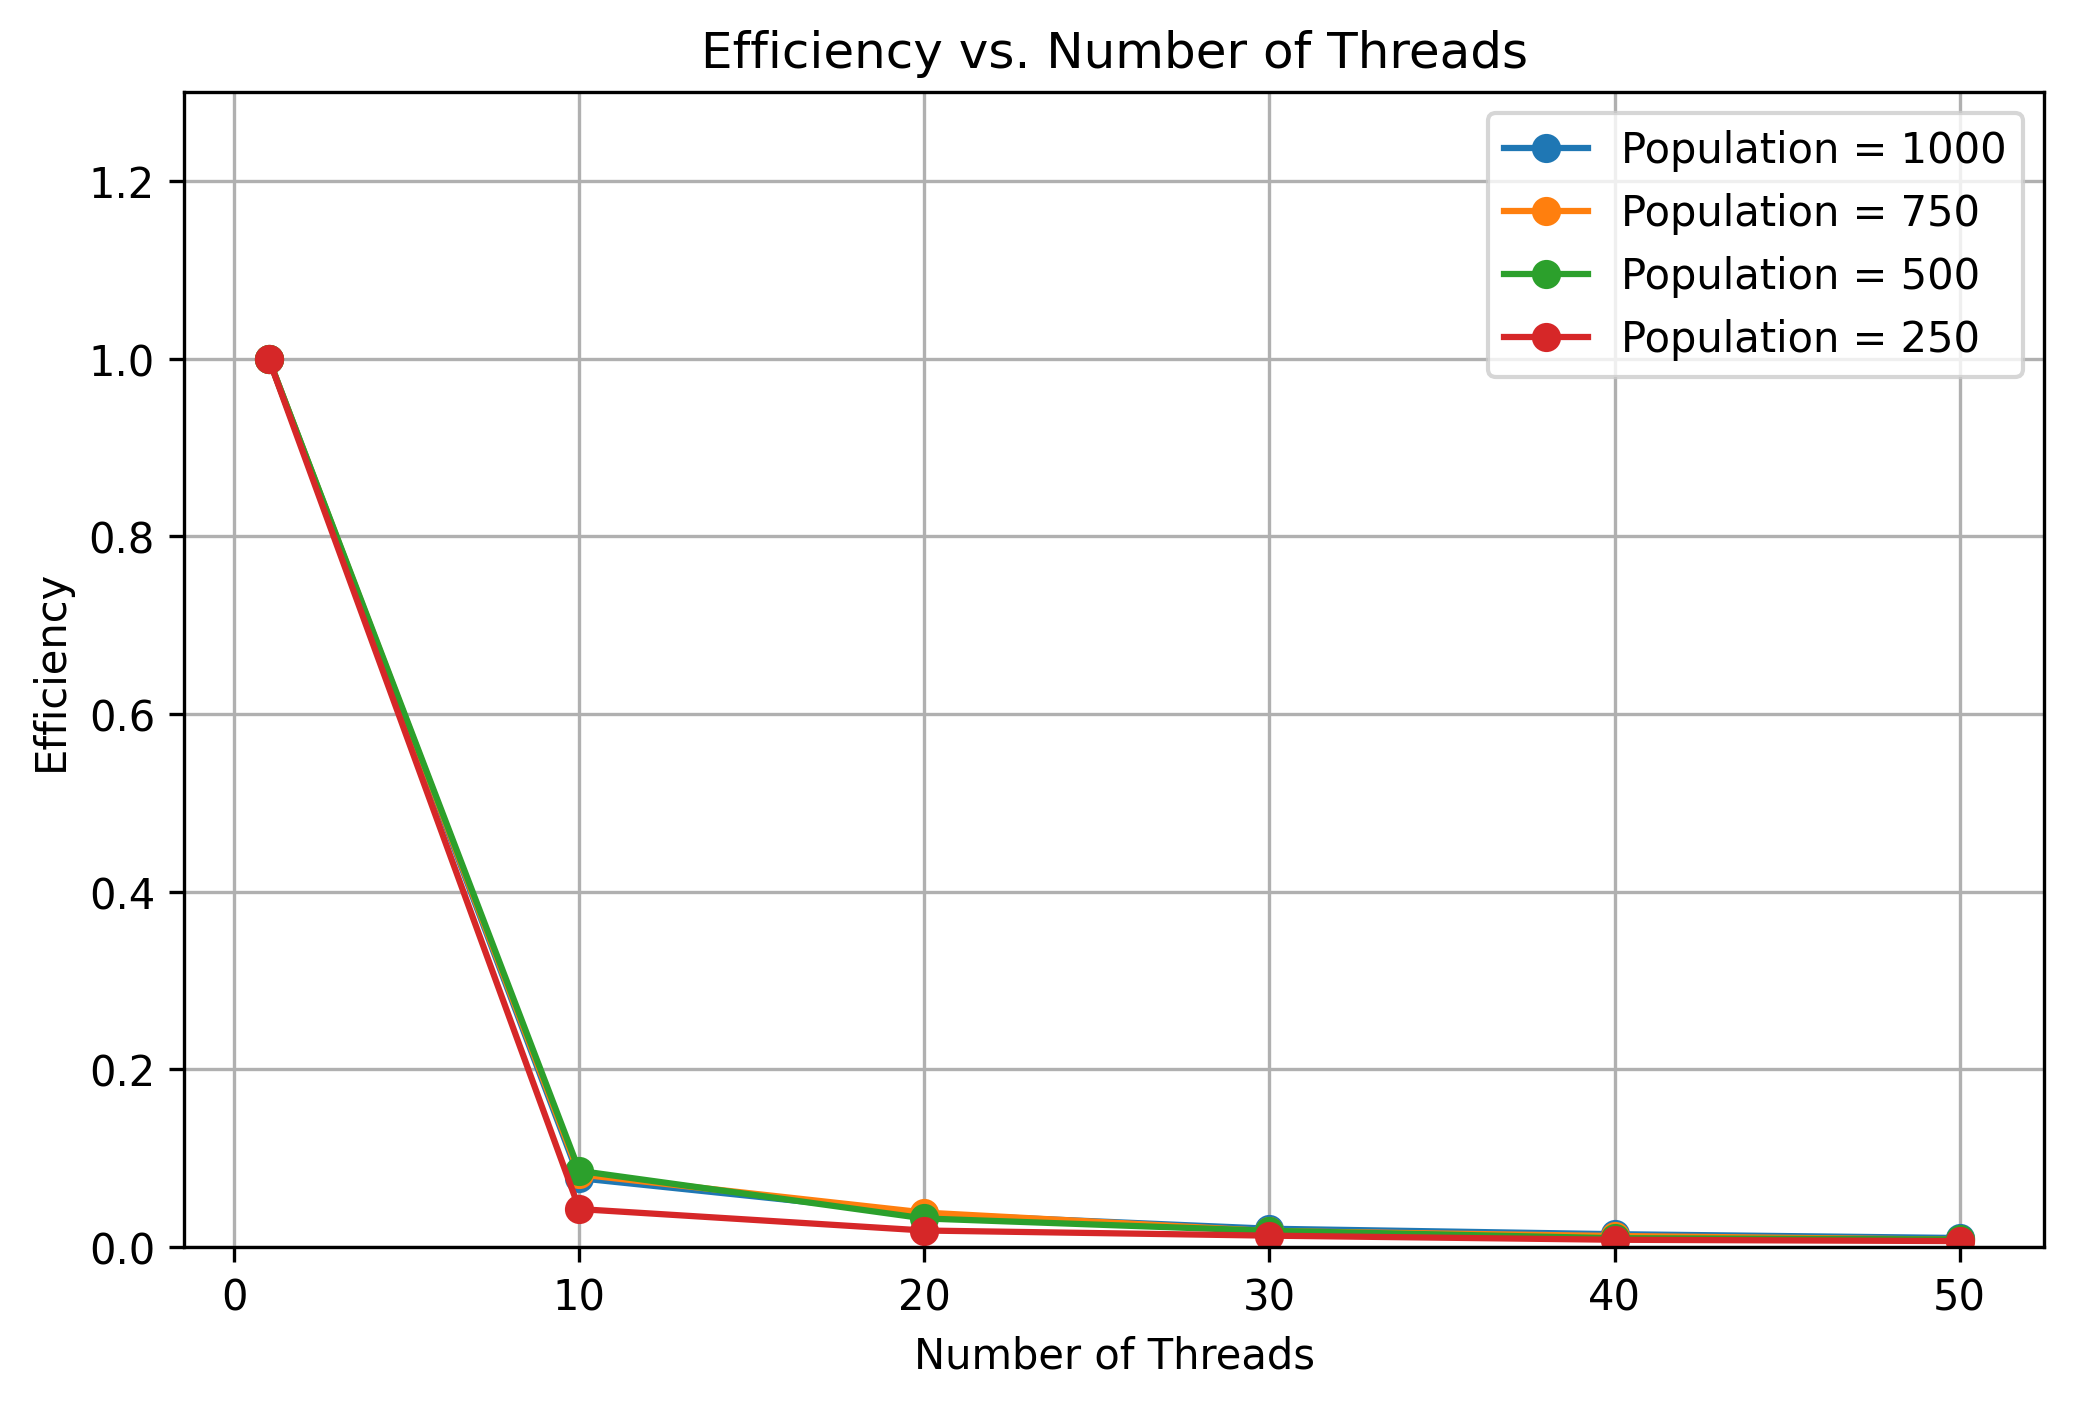
\includegraphics[width=\linewidth]{figures/efficiency_vs_threads.png}
        \caption{Efficiency vs. Number of Threads}
    \end{subfigure}
    \caption{Performance analysis using increasing number of threads.}
    \label{fig:nodes_performance}
\end{figure}
\newline
\subsection{Multithreaded Performance Degradation}
Despite our expectation that multithreading would improve performance, the \textbf{OpenMP} implementation resulted in significant degradation compared to the sequential version. Several potential factors may contribute to this behavior:

\begin{itemize}
    \item \textbf{Scheduling Overhead:} We used dynamic scheduling, which generally introduces more overhead than static scheduling when the workload per thread is uniform. However, extensive empirical testing showed that, despite the relatively even distribution of workload, the dynamic scheduling strategy consistently outperformed static scheduling.

    \item \textbf{False Sharing:} If threads update data stored in contiguous memory locations, cache line contention may occur, leading to performance loss. This could be the case for the temporary arrays allocated per thread, potentially causing frequent cache invalidations.

    \item \textbf{Memory Bandwidth Constraints:} Frequent updates to large data structures might be saturating the available memory bandwidth, making the algorithm memory-bound. This effect could be exacerbated by dynamic memory allocation, which may introduce additional overhead due to inefficient memory access patterns.

    \item \textbf{Granularity of Computation:} The computational load per thread may be too small to offset the overhead associated with thread management, leading to inefficient parallel execution.

    \item \textbf{Allocation Overhead:} Although temporary arrays are allocated outside the parallel loop, their allocation strategy or memory alignment might still impact performance, particularly if memory fragmentation occurs.
\end{itemize}

Despite extensive testing and multiple modifications to the parallel implementation, we were unable to definitively determine the exact cause of the performance degradation. Further profiling and targeted optimizations (e.g., adjusting memory allocation strategies, reducing false sharing, and analyzing cache behavior) are necessary to gain deeper insights into the issue.
